\chapter{Rupture spontanée de la supersymétrie et premier multiplet \texorpdfstring{\(SU(5)\)}{SU(5)}}

\lectureoverview{La rupture de symétrie apparaît d’abord ici comme un fait visible dans les spectres : les niveaux d’un atome invariant par rotation sont dégénérés, tandis qu’un champ magnétique les sépare. Un ferromagnétique enseigne ensuite une leçon plus subtile : les équations peuvent conserver une symétrie que le vide, lui, ne possède pas. Des magnons sans gap, la condition \(J|0\rangle\neq0\) et un paramètre d’ordre non nul sont trois façons de décrire ce même phénomène. Nous transposons ce schéma dans une théorie des champs supersymétrique chirale, dérivons le potentiel scalaire \(V=|W'|^2\) en éliminant le champ auxiliaire \(F\), et distinguons les vides supersymétriques de ceux où la supersymétrie est brisée par \(F\). L’énergie du vide qui en résulte, la séparation entre bosons--fermions, le goldstino, le secteur caché et le mécanisme super-Higgs achèvent la discussion de la supersymétrie. La dernière partie change de sujet et introduit la grande unification : \(SU(3)\times SU(2)\times U(1)\) est plongé bloc par bloc dans \(SU(5)\), dont le premier multiplet de matière réunit un doublet de leptons et trois antiquarks down.}

\section{Un spectre garde la trace de sa symétrie}

Commencer par un atome ne vise pas simplement à réviser les notions élémentaires de mécanique quantique. Les niveaux d’énergie et les masses des particules sont des données spectrales de même nature. Si une symétrie impose l’égalité de niveaux atomiques, sa rupture peut les séparer ; en théorie des champs, cela signifie que les membres d’un multiplet de particules peuvent acquérir des masses différentes.

Considérons un état atomique de moment cinétique total \(j\), qui comprend les contributions du spin et du moment orbital. Par rapport à un axe choisi,
\begin{equation}
J_z|j,m\rangle=m\hbar|j,m\rangle,
\qquad
m=-j,-j+1,\ldots,j,
\end{equation}
il existe donc \(2j+1\) états. Les flèches familières des manuels ne signifient pas que le vecteur moment cinétique n’a littéralement que \(2j+1\) directions spatiales possibles. C’est sa composante selon l’axe choisi qui est quantifiée.

Dans le vide, en espace invariant par rotation, rien ne justifie de privilégier cet axe. Une rotation mélange les états du multiplet de spin-\(j\), et l’invariance de l’hamiltonien implique
\begin{equation}
[H,\mathbf J]=0,
\qquad
E_{j,-j}=E_{j,-j+1}=\cdots=E_{j,j}.
\label{eq:l9-degeneracy}
\end{equation}

\begin{classroomqa}\audiencequestion{Quelle symétrie garantit que la rotation de l’atome tout entier ne peut pas modifier son énergie ? \lecturetimestamp{00:05:53}}\lecturerresponse{La symétrie de rotation. Comme une rotation transforme une orientation du moment cinétique en une autre sans modifier le système physique, les \(2j+1\) états ont tous la même énergie.}\end{classroomqa}

Appliquons maintenant un champ magnétique \(\mathbf B=B\hat{\mathbf z}\). L’interaction
\begin{equation}
H_B=-\boldsymbol{\mu}\cdot\mathbf B
\end{equation}
distingue la composante parallèle au champ. Schématiquement,
\begin{equation}
\Delta E_m\propto mB.
\label{eq:l9-zeeman}
\end{equation}
À faible champ, les niveaux correspondant à différentes valeurs de \(m\) se séparent linéairement, et les transitions entre eux dédoublent les raies spectrales.

\begin{classroomqa}\audiencequestion{Comment appelle-t-on la séparation des niveaux atomiques dans un champ magnétique ? \lecturetimestamp{00:07:13}}\lecturerresponse{L’effet Zeeman. C’est le prototype de toute la discussion : des niveaux rendus dégénérés par une symétrie se séparent lorsqu’un champ de fond brise cette symétrie.}\end{classroomqa}

\begin{center}
\begin{tikzpicture}[x=1.05cm,y=0.75cm,>=Latex]
  \draw[thick] (-3,0) -- (-1,0);
  \node[left] at (-3,0) {\(B=0\)};
  \foreach \y/\m in {-1.2/-1,-0.4/0,0.4/1,1.2/2} {
    \draw[thick,teal!70!black] (1,\y) -- (3,\y);
    \node[right] at (3,\y) {\(m=\m\)};
  }
  \draw[->,thick] (-0.5,0) -- (0.6,0);
  \node[above] at (0.05,0) {\(\mathbf B\neq0\)};
\end{tikzpicture}
\end{center}

\section{Le ferromagnétique : lois symétriques, vide asymétrique}

Dans un modèle microscopique simple d’un ferromagnétique, chaque site porte un petit moment magnétique. Si les moments voisins abaissent leur énergie en s’alignant parallèlement, la phase à basse température est ferromagnétique. Si l’alignement antiparallèle est favorisé, on obtient un antiferromagnétique. De fortes fluctuations thermiques ou quantiques peuvent au contraire effacer toute aimantation nette.

Supposons qu’un ferromagnétique remplisse le monde et se stabilise dans un état uniformément aligné. Son champ magnétique interne sépare les niveaux d’un atome comme le ferait un champ appliqué de l’extérieur. Mais une différence décisive subsiste. Les interactions sous-jacentes ne privilégient ni le nord, ni l’est, ni aucune autre direction. Toutes les configurations uniformes obtenues par rotation ont la même énergie :
\begin{equation}
\mathbf M(\mathbf x)=M_0\hat{\mathbf n},
\qquad
\hat{\mathbf n}\in S^2.
\label{eq:l9-ferromagnetic-vacua}
\end{equation}
Les équations sont invariantes par rotation, mais un état fondamental donné choisit une direction \(\hat{\mathbf n}\). La rupture de symétrie est spontanée, et non explicite.

Un habitant constitué d’excitations de ce milieu ne peut pas saisir l’univers entier pour le faire tourner. À l’échelle locale, la direction choisie semble donc aussi fondamentale qu’un champ extérieur. L’atome voit toujours le même schéma de niveaux, son moment cinétique étant projeté selon \(\hat{\mathbf n}\) plutôt que selon un axe \(z\) désigné de l’extérieur. La question est de savoir comment un observateur interne pourrait découvrir que l’asymétrie apparente appartient à l’état, et non aux lois.

\subsection{Le critère de Goldstone}

Une rotation uniforme de tous les moments fait passer d’un vide à un autre dans l’équation~\eqref{eq:l9-ferromagnetic-vacua}, sans coût énergétique. Faisons plutôt varier très progressivement l’orientation dans l’espace. Les moments voisins exercent alors les uns sur les autres des forces qui propagent la déformation sous la forme d’une onde de spin, dont les quanta sont les magnons. Lorsque la longueur d’onde tend vers l’infini, la configuration se rapproche d’une rotation uniforme et l’énergie de l’excitation tend vers zéro :
\begin{equation}
k=\frac{2\pi}{\lambda}\longrightarrow0
\quad\Longrightarrow\quad
E(k)\longrightarrow0.
\label{eq:l9-gapless-magnon}
\end{equation}
Deux habitants peuvent faire osciller des moments voisins, envoyer de telles ondes à travers le milieu et mesurer cette énergie arbitrairement faible. Cette expérience révèle la rupture spontanée, même s’ils ne peuvent pas faire tourner le monde.

\editorialnote{Un magnon ferromagnétique est sans gap, mais sa relation de dispersion est généralement quadratique et non relativiste, \(E\propto k^2\), plutôt que la relation relativiste \(E\propto|k|\). Dans cette conférence, le terme « sans masse » désigne le sens physiquement pertinent d’un gap nul. Dans les deux cas, il s’agit de modes de Goldstone.}

La même idée s’applique aux symétries internes continues, notamment aux groupes de jauge et de saveur de la physique des particules. Toutefois, lorsque la symétrie brisée est jaugée, le mode de Goldstone ne subsiste pas comme particule sans masse indépendante.

\begin{classroomqa}\audiencequestion{Que se passe-t-il lorsqu’on combine la brisure spontanée de symétrie avec l’invariance de jauge ? \lecturetimestamp{00:15:56}}\lecturerresponse{Le boson de Goldstone fournit une polarisation supplémentaire au champ de jauge. Le boson de jauge devient massif : c’est le mécanisme de Higgs, auquel nous reviendrons dans l’analogie gravitationnelle.}\end{classroomqa}

\section{Trois signes équivalents de la brisure}

On peut désormais décrire le ferromagnétique dans trois langages qui se renforcent mutuellement.

\paragraph{Des vides dégénérés.}
Il existe un état d’énergie minimale pour chaque orientation \(\hat{\mathbf n}\). La physique se déroule dans l’un des membres choisis de cette famille, bien que la symétrie les relie tous.

\paragraph{Un générateur qui n’annule pas le vide.}
Soit \(J_a\) un générateur des rotations. Une transformation finie s’écrit
\begin{equation}
U(\epsilon)=e^{-i\epsilon J_a},
\end{equation}
et \(J_a|0\rangle\) est proportionnel à la variation infinitésimale du vide, et non à l’état entièrement tourné.

\begin{classroomqa}\audiencequestion{Quels sont les générateurs de la symétrie de rotation ? \lecturetimestamp{00:17:29}}\lecturerresponse{Les composantes du moment cinétique total. Nous les appelons \(J_a\) parce qu’elles font tourner tout ce qui se trouve dans l’état, et pas seulement un atome.}\end{classroomqa}

Un générateur non brisé satisfait
\begin{equation}
J_a|0\rangle=0.
\label{eq:l9-unbroken-generator}
\end{equation}
Un générateur brisé donne au contraire
\begin{equation}
J_a|0\rangle\neq0.
\label{eq:l9-broken-generator}
\end{equation}

\begin{classroomqa}\audiencequestion{Si \(J_a|0\rangle\) est non nul, donne-t-il simplement le même vide ? \lecturetimestamp{00:19:43}}\lecturerresponse{Non. Il donne la différence infinitésimale entre le vide choisi et un vide légèrement tourné. Physiquement, cette différence correspond à une excitation de Goldstone de longueur d’onde infinie.}\end{classroomqa}

\begin{classroomqa}\audiencequestion{Cette rotation infinitésimale modifie-t-elle l’énergie ? \lecturetimestamp{00:20:14}}\lecturerresponse{Non. Le vide tourné est dégénéré avec le vide initial ; l’état de Goldstone à impulsion nulle a donc une énergie nulle.}\end{classroomqa}

Symboliquement,
\begin{equation}
J_a|0\rangle
\sim
|\pi_a,\mathbf k=0\rangle,
\label{eq:l9-generator-goldstone}
\end{equation}
où \(\pi_a\) désigne le mode de Goldstone associé au générateur brisé.

\paragraph{Un paramètre d’ordre non nul.}
L’aimantation locale \(\mathbf M(\mathbf x)\) est un champ. Dans une phase chaude ou désordonnée quantiquement,
\begin{equation}
\langle\mathbf M\rangle=0,
\end{equation}
et le vide ne sélectionne aucune direction. Dans la phase ordonnée,
\begin{equation}
\langle M_i\rangle\neq0
\quad\text{for at least one component }i,
\label{eq:l9-magnetization-order}
\end{equation}
une rotation mélange donc cette composante non nulle aux autres. Les vides dégénérés, un générateur brisé et un paramètre d’ordre non nul sont les trois schémas que nous allons transposer à la supersymétrie.

\section{Rappel sur le multiplet chiral}

L’exemple le plus simple en quatre dimensions contient un scalaire complexe, un fermion de Weyl et un scalaire complexe auxiliaire. En coordonnées chirales,
\begin{equation}
y^\mu=x^\mu+i\bar\theta\bar\sigma^\mu\theta,
\end{equation}
un superchamp chiral peut se développer schématiquement sous la forme
\begin{equation}
\Phi(y,\theta)=
\phi(y)+\sqrt2\,\theta\psi(y)+\theta^2F(y).
\label{eq:l9-chiral-expansion}
\end{equation}
La conférence omet le facteur conventionnel \(\sqrt2\) ; nous l’inclurons désormais afin que les coefficients des composantes soient ceux de la convention standard. Un superchamp chiral est intrinsèquement complexe : imposer la réalité n’est pas préservé par sa transformation supersymétrique.

L’action cinétique supersymétrique est
\begin{equation}
S_{\mathrm{kin}}
=
\int d^4x\,d^4\theta\,
\Phi^\dagger\Phi.
\label{eq:l9-kahler-action}
\end{equation}
L’intégration de Grassmann sélectionne le coefficient de
\(\theta^2\bar\theta^2\). Avec la métrique de signature principalement négative, le résultat en composantes est
\begin{equation}
\mathcal L_{\mathrm{kin}}
=
\partial_\mu\phi^\ast\,\partial^\mu\phi
+i\bar\psi\bar\sigma^\mu\partial_\mu\psi
+F^\ast F.
\label{eq:l9-chiral-kinetic}
\end{equation}
Les deux premiers termes décrivent la propagation du scalaire et du fermion. Le dernier ne contient pas de dérivée et ne décrit donc la propagation d’aucune particule.

\begin{figure}[H]\centering
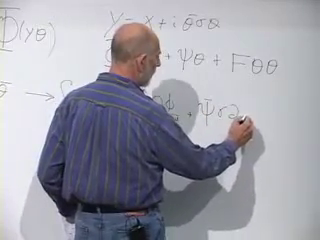
\includegraphics[width=0.76\textwidth]{lecture_09_figure_02.png}\lectureframe{00:27:36.000}\caption{La coordonnée chirale et le développement en composantes, au-dessus des termes du scalaire, du fermion et du champ auxiliaire.}\end{figure}

\section{Ce que sélectionne l’intégrale \texorpdfstring{\(d^2\theta\)}{d2-theta}}

Les interactions et les masses proviennent d’une fonction holomorphe \(W(\Phi)\), le superpotentiel :
\begin{equation}
S_W
=
\int d^4x
\left[
\int d^2\theta\,W(\Phi)
+\mathrm{h.c.}
\right].
\label{eq:l9-superpotential-action}
\end{equation}
Une expression chirale ne dépend pas de manière indépendante de \(\bar\theta\) ; son intégration sur les quatre coordonnées impaires donnerait donc zéro. L’intégrale \(d^2\theta\) sélectionne plutôt sa composante \(\theta^2\).

Pour voir les facteurs combinatoires avant de considérer une fonction générale, prenons \(W(\Phi)=\Phi^n\). Dans
\begin{equation}
(\phi+\sqrt2\,\theta\psi+\theta^2F)^n,
\end{equation}
il existe deux façons d’obtenir exactement deux facteurs \(\theta\). On peut choisir un seul facteur \(F\theta^2\) ou choisir deux facteurs fermioniques.

\begin{classroomqa}\audiencequestion{Combien de termes contiennent un facteur \(F\theta^2\) choisi, et seulement des scalaires par ailleurs : \(n-1\) ou \(n\) ? \lecturetimestamp{00:31:33}}\lecturerresponse{Il y en a \(n\). N’importe lequel des facteurs \(n\) peut fournir \(F\theta^2\) ; les \(n-1\) facteurs restants fournissent \(\phi\). La contribution est \(nF\phi^{n-1}\).}\end{classroomqa}

\begin{classroomqa}\audiencequestion{De combien de façons deux facteurs peuvent-ils fournir les deux fermions ? \lecturetimestamp{00:32:26}}\lecturerresponse{Il y a \(\binom n2=n(n-1)/2\) choix sans ordre. La contraction de Grassmann fixe le terme correspondant en \(\psi\psi\).}\end{classroomqa}

Ainsi, dans la notation de la conférence où les coefficients sont omis,
\begin{equation}
\int d^2\theta\,\Phi^n+\mathrm{h.c.}
\;\leadsto\;
nF\phi^{n-1}
-\frac{n(n-1)}{2}\phi^{n-2}\psi\psi
+\mathrm{h.c.}
\label{eq:l9-power-extraction}
\end{equation}
Le signe moins affiché ici découle du développement normalisé standard et de la convention de Grassmann ; un changement de convention peut modifier les signes apparents.

\begin{classroomqa}\audiencequestion{Qu’est-il advenu du terme \(\phi^n\), qui ne contient aucun facteur \(\theta\) ? \lecturetimestamp{00:33:10}}\lecturerresponse{Il figure bien dans le produit, mais l’intégration \(d^2\theta\) l’élimine. La flèche signifie que l’intégration sélectionne le coefficient de \(\theta^2\) ; elle n’exprime pas l’égalité des expressions complètes.}\end{classroomqa}

\begin{figure}[H]\centering
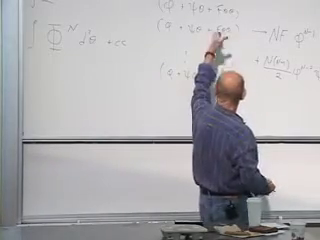
\includegraphics[width=0.82\textwidth]{lecture_09_figure_03.png}\lectureframe{00:33:38.000}\caption{Les facteurs répétés de superchamp et la flèche d’implication, qui extrait la composante en deux facteurs \(\theta\) au lieu de lui être égale.}\end{figure}

La somme des puissances affectées de coefficients arbitraires transforme les facteurs combinatoires en dérivées :
\begin{equation}
\int d^2\theta\,W(\Phi)+\mathrm{h.c.}
\;\leadsto\;
F W'(\phi)
-\frac12 W''(\phi)\psi\psi
+\mathrm{h.c.}
\label{eq:l9-W-components}
\end{equation}

\begin{classroomqa}\audiencequestion{Pourquoi le terme fermionique contient-il \(\phi^{n-2}\) plutôt que \(\phi^{n-1}\) ? \lecturetimestamp{00:36:32}}\lecturerresponse{Deux facteurs ont déjà fourni les fermions ; il reste donc \(n-2\) facteurs scalaires. Le coefficient est la moitié de la dérivée seconde \(W''(\phi)\).}\end{classroomqa}

Le terme fermionique est important : il produit une masse lorsque \(W''\) est constant et une interaction de Yukawa lorsque \(W''\) dépend de \(\phi\). Pour analyser le vide, toutefois, le terme auxiliaire \(FW'\) fournit immédiatement les informations utiles.

\section{Élimination du champ auxiliaire}

Rassemblons les termes qui contiennent \(F\) :
\begin{equation}
\mathcal L_F
=
F^\ast F
+F W'(\phi)
+F^\ast \overline{W'(\phi)}.
\label{eq:l9-LF}
\end{equation}
Comme il n’y a pas de terme \(\partial_\mu F\), l’équation complète d’Euler--Lagrange
\begin{equation}
\partial_\mu
\frac{\partial\mathcal L}{\partial(\partial_\mu F)}
-
\frac{\partial\mathcal L}{\partial F}
=0
\end{equation}
se réduit immédiatement à une équation algébrique. En traitant \(F\) et \(F^\ast\) comme des variables indépendantes, on obtient
\begin{align}
\frac{\partial\mathcal L_F}{\partial F}
&=F^\ast+W'(\phi)=0,
&
\frac{\partial\mathcal L_F}{\partial F^\ast}
&=F+\overline{W'(\phi)}=0,
\label{eq:l9-F-eom}
\end{align}
et donc
\begin{equation}
F^\ast=-W'(\phi),
\qquad
F=-\overline{W'(\phi)}.
\label{eq:l9-F-solution}
\end{equation}

\begin{figure}[H]\centering
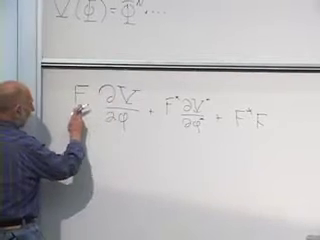
\includegraphics[width=0.82\textwidth]{lecture_09_figure_04.png}\lectureframe{00:39:40.000}\caption{L’expression complète faisant intervenir le champ auxiliaire et son équation du mouvement algébrique, visibles ensemble une fois le tableau dégagé.}\end{figure}

\begin{classroomqa}\audiencequestion{Cette dérivée ne devrait-elle pas être prise par rapport à \(\phi\), plutôt qu’au champ conjugué indiqué au tableau ? \lecturetimestamp{00:41:21}}\lecturerresponse{Oui. La correction rétablit la paire de champs conjugués dans l’équation~\eqref{eq:l9-F-eom} : \(F^\ast=-W'(\phi)\) et \(F=-\overline{W'(\phi)}\).}\end{classroomqa}

La substitution dans l’équation~\eqref{eq:l9-LF} donne
\begin{equation}
\mathcal L_F\big|_{\mathrm{on\ shell}}
=-|W'(\phi)|^2.
\end{equation}
Comme un lagrangien scalaire est égal à l’énergie cinétique moins l’énergie potentielle, le potentiel scalaire usuel est
\begin{equation}
\boxed{V(\phi,\phi^\ast)=|W'(\phi)|^2\ge0.}
\label{eq:l9-F-potential}
\end{equation}
Ce \(V\) n’est pas le superpotentiel. Nous réservons \(W\) à la fonction holomorphe de l’espace supersymétrique et \(V\) à l’énergie potentielle usuelle.

\subsection{Deux exemples immédiats}

Avec les normalisations conventionnelles exactes,
\begin{equation}
\begin{gathered}
W(\Phi)=\frac12m\Phi^2,\\
W'(\phi)=m\phi,
\qquad V=|m|^2|\phi|^2.
\end{gathered}
\label{eq:l9-quadratic-W}
\end{equation}
Le même terme donne la masse du fermion,
\(-\tfrac12m\psi\psi+\mathrm{h.c.}\)
si bien que les masses du scalaire et du fermion sont égales avant la brisure de la supersymétrie.

Pour
\begin{equation}
W(\Phi)=\frac{g}{3}\Phi^3,
\end{equation}
on obtient
\begin{equation}
\begin{gathered}
W'(\phi)=g\phi^2,
\qquad V=|g|^2|\phi|^4,\\
\mathcal L_{\mathrm{Yukawa}}
=-g\phi\psi\psi+\mathrm{h.c.}
\end{gathered}
\label{eq:l9-cubic-W}
\end{equation}
Le vertex scalaire quartique décrit la diffusion de deux scalaires, tandis que le terme de Yukawa en est le partenaire supersymétrique.

\section{Deux types de vide}

Le vide est une configuration de champ constante correspondant à un minimum de \(V\) ; les termes dérivés s’annulent. Comme l’équation~\eqref{eq:l9-F-potential} est non négative, deux cas sont possibles.

\subsection{Un minimum d’énergie nulle}

Si un certain \(\phi_0\) satisfait
\begin{equation}
W'(\phi_0)=0,
\end{equation}
alors
\begin{equation}
V(\phi_0)=0,
\qquad
\langle F\rangle=0.
\label{eq:l9-unbroken-F}
\end{equation}
Le vide est supersymétrique. C’est l’analogue d’une aimantation nulle : aucune composante auxiliaire n’a sélectionné de direction dans l’espace supersymétrique.

\subsection{Un minimum relevé}

Si les équations
\begin{equation}
W'(\phi)=0
\label{eq:l9-F-flatness}
\end{equation}
n’ont pas de solution simultanée au minimum, alors
\begin{equation}
V_{\min}>0,
\qquad
\langle F\rangle\neq0,
\label{eq:l9-broken-F}
\end{equation}
et la supersymétrie est spontanément brisée. L’action demeure supersymétrique ; son état d’énergie minimale, lui, ne l’est pas.

\begin{figure}[H]\centering
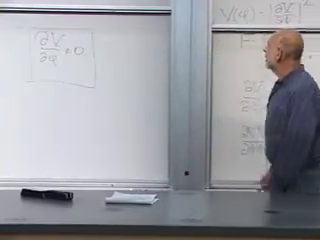
\includegraphics[width=0.88\textwidth]{lecture_09_figure_05.png}\lectureframe{00:52:09.960}\caption{Le tableau présente le potentiel positif, l’équation en \(F\) et la condition sur le vide, tout en distinguant des équations symétriques une solution qui ne l’est pas.}\end{figure}

L’énoncé concernant le paramètre d’ordre se précise à partir de la transformation du fermion :
\begin{equation}
\delta\psi_\alpha
=
i\sqrt2
(\sigma^\mu\bar\epsilon)_\alpha\partial_\mu\phi
+\sqrt2\,\epsilon_\alpha F.
\label{eq:l9-fermion-transformation}
\end{equation}
Dans un vide homogène, le terme dérivé s’annule. Si
\(\langle F\rangle\neq0\), la supersymétrie décale le fermion d’une constante non nulle, de sorte que le vide ne peut pas être invariant.\editorialnote{L’équation~\eqref{eq:l9-fermion-transformation} est la forme standard en composantes qui explicite l’énoncé de la conférence selon lequel les composantes du superchamp se transforment les unes en les autres.}

La même conclusion découle de la superalgèbre. Dans le référentiel au repos,
\begin{equation}
\{Q_\alpha,Q_{\dot\alpha}^\dagger\}
=2\sigma^0_{\alpha\dot\alpha}H.
\end{equation}
La valeur moyenne dans le vide exprime son énergie comme une somme des normes des charges de supersymétrie appliquées au vide :
\begin{equation}
E_0\ge0,
\qquad
E_0=0
\ \Longleftrightarrow\
Q_\alpha|0\rangle
=Q_{\dot\alpha}^\dagger|0\rangle=0.
\label{eq:l9-algebra-vacuum-energy}
\end{equation}
Ainsi, une énergie positive du vide et la brisure spontanée de la supersymétrie sont deux aspects d’un même énoncé en supersymétrie globale.

\begin{center}
\begin{tikzpicture}[x=1.2cm,y=1.0cm,>=Latex]
  \draw[->] (-3,0) -- (-0.2,0) node[right] {\(\phi\)};
  \draw[->] (-2.8,-0.15) -- (-2.8,2.1) node[above] {\(V\)};
  \draw[thick,teal!75!black,domain=-2.5:-0.5,samples=60]
    plot (\x,{0.65*(\x+1.5)^2});
  \fill (-1.5,0) circle (2pt);
  \node[below] at (-1.5,0) {\(F=0\)};
  \draw[->] (0.4,0) -- (3.2,0) node[right] {\(\phi\)};
  \draw[->] (0.6,-0.15) -- (0.6,2.1) node[above] {\(V\)};
  \draw[thick,orange!85!black,domain=0.9:2.9,samples=60]
    plot (\x,{0.55*(\x-1.9)^2+0.65});
  \fill (1.9,0.65) circle (2pt);
  \draw[dashed] (0.6,0.65) -- (1.9,0.65);
  \node[below] at (1.9,0.65) {\(F\neq0\)};
\end{tikzpicture}
\end{center}

\editorialnote{Une illustration minimale est donnée par \(W=f\Phi\), pour laquelle \(W'=f\) ne s’annule jamais et \(V=|f|^2\). Cet exemple à un seul champ présente une direction scalaire plate ; en pratique, la brisure stable par terme \(F\) se réalise généralement au moyen de plusieurs champs chiraux, comme dans les secteurs cachés de type O’Raifeartaigh.}

\section{Ce que produit la brisure de la supersymétrie}

\subsection{Séparation des masses}

L’analogie avec le ferromagnétique redevient spectrale. Un faible champ magnétique interne sépare les niveaux atomiques sans détruire l’identité de l’atome. De même, un paramètre d’ordre associé à la brisure de la supersymétrie, transmis par couplage faible, sépare les bosons et les fermions qui appartiendraient autrement à un même supermultiplet.

\begin{classroomqa}\audiencequestion{Quelles particules la supersymétrie transforme-t-elle les unes en les autres et perdent ainsi leur dégénérescence de masse lorsque le vide brise cette symétrie ? \lecturetimestamp{00:51:40}}\lecturerresponse{Les bosons et les fermions. Leurs masses n’ont plus besoin d’être égales dès lors que l’état ne respecte plus la transformation qui les relie.}\end{classroomqa}

La séparation n’est pas produite par \(\langle F\rangle\) à lui seul ; elle dépend des couplages qui transmettent la brisure aux champs visibles. Si ces couplages sont faibles, les particules visibles restent reconnaissables et les écarts de masse sont petits devant les échelles de grande unification ou de Planck. S’ils étaient forts, l’analogie serait celle d’un atome tellement déformé par un champ magnétique immense qu’il deviendrait un objet allongé et méconnaissable.

\subsection{Le goldstino}

Pour un générateur ordinaire brisé, \(J|0\rangle\) donne un état de Goldstone bosonique. Une charge de supersymétrie est fermionique et transforme les états bosoniques en états fermioniques. Puisque le vide est compté comme bosonique, une charge de supersymétrie brisée crée un état fermionique d’énergie nulle :
\begin{equation}
Q_\alpha|0\rangle
\sim
|\widetilde G_\alpha,\mathbf k=0\rangle.
\label{eq:l9-goldstino}
\end{equation}
La particule correspondante en propagation est un fermion de Weyl sans masse, le fermion de Goldstone, ou goldstino.

\begin{classroomqa}\audiencequestion{Si une transformation supersymétrique ne laisse pas le vide inchangé, quel nouvel état crée-t-elle ? \lecturetimestamp{00:53:24}}\lecturerresponse{Un fermion sans masse. Le schéma du théorème de Goldstone ordinaire subsiste, mais un générateur fermionique transforme le vide bosonique en goldstino.}\end{classroomqa}

La brisure spontanée d’une supersymétrie globale a donc deux signatures inévitables :
\begin{equation}
\boxed{
V_{\min}>0
\qquad\text{and}\qquad
\text{a massless goldstino}.
}
\label{eq:l9-rigid-breaking-signatures}
\end{equation}

\section{Le secteur caché}

Il est utile de considérer l’atome et le ferromagnétique comme deux secteurs. Le ferromagnétique développe le paramètre d’ordre ; l’atome ne ressent que le champ qui lui est transmis. Lorsque le couplage est faible, manipuler l’atome excite à peine un magnon et donne peu d’accès direct au milieu magnétique. Le ferromagnétique est alors caché, même si sa présence se déduit de faibles écarts spectraux.

La construction de modèles supersymétriques reprend le même vocabulaire. Des champs supplémentaires d’un secteur caché développent des valeurs moyennes non nulles des termes \(F\) ou \(D\). Des interactions, dites mécanisme de médiation, transmettent cette brisure au secteur visible et engendrent des masses molles pour les partenaires supersymétriques. Une transmission faible explique comment la théorie visible peut rester approximativement supersymétrique à une échelle fondamentale bien plus élevée, tout en ne présentant aucune dégénérescence exacte entre bosons--fermions à basse énergie.

Cette construction ne se fait pas automatiquement. Il faut des champs supplémentaires, un vide de brisure stable et un mécanisme de médiation contrôlé. C’est pourquoi la conférence décrit la brisure réaliste de la supersymétrie comme compliquée et quelque peu artificielle, plutôt que comme une conséquence unique et inévitable du modèle minimal.

\section{La gravité modifie les deux signatures}

\subsection{L’énergie du vide devient une source}

En l’absence de gravité, ajouter une constante à toutes les énergies ne modifie pas les expériences non gravitationnelles. En présence de gravité, une densité d’énergie du vide intervient dans l’équation d’Einstein comme constante cosmologique. Un \(V_{\min}\) positif entraîne une expansion accélérée. Si son échelle était comparable à celle de la physique des particules requise pour les masses des partenaires supersymétriques, la courbure qui en résulterait serait immensément supérieure à celle qui est observée.

\begin{classroomqa}\audiencequestion{Que fait au monde une énergie du vide positive et non nulle lorsque l’on tient compte de la gravité ? \lecturetimestamp{01:00:40}}\lecturerresponse{Elle agit comme une constante cosmologique et entraîne une expansion accélérée. Aux échelles usuelles de la physique des particules, son effet serait intolérablement important.}\end{classroomqa}

La supersymétrie locale, ou supergravité, modifie la formule exprimant le potentiel comme un carré positif. Pour fixer les idées, le potentiel standard associé aux termes \(N=1\) \(F\) s’écrit
\begin{equation}
\begin{aligned}
V_F={}&e^{K/M_P^2}
\left(
K^{i\bar j}D_iW\,D_{\bar j}\overline W
-\frac{3|W|^2}{M_P^2}
\right),\\
D_iW={}&\partial_iW+\frac{\partial_iK}{M_P^2}W.
\end{aligned}
\label{eq:l9-sugra-potential}
\end{equation}
En raison du terme négatif, l’énergie positive due à la brisure de la supersymétrie peut en principe être partiellement compensée. Le résidu peut correspondre à une faible constante cosmologique.

\editorialnote{La conférence ne donne volontairement qu’une correction schématique et met explicitement en doute la position de la masse de Planck. L’équation~\eqref{eq:l9-sugra-potential} donne la formule conventionnelle pour des multiplets chiraux de potentiel de Kähler \(K\) ; les termes de jauge \(D\) ajouteraient une contribution supplémentaire non négative. Elle n’explique pas la valeur infime observée, qui reste le problème de la constante cosmologique.}

\subsection{Le mécanisme super-Higgs}

Le second effet gravitationnel se comprend le plus facilement en comptant les polarisations. Une particule massive de spin-\(j\) possède \(2j+1\) états de spin dans son référentiel au repos.

\begin{classroomqa}\audiencequestion{Combien d’états de spin possède une particule massive de spin-\(j\) ? \lecturetimestamp{01:05:16}}\lecturerresponse{\(2j+1\). Une particule massive de spin un possède notamment trois états, tandis qu’un boson de jauge sans masse n’a que les hélicités \(+1\) et \(-1\).}\end{classroomqa}

La distinction est cinématique. On peut appliquer un boost à une particule massive pour la mettre au repos, puis la diriger dans une nouvelle direction tout en conservant l’orientation de son spin ; toutes les projections doivent donc exister. Une particule sans masse ne peut être dépassée ni mise au repos. Elle ne peut donc porter que les deux hélicités extrêmes.

Pour le champ de jauge électrofaible,
\begin{equation}
\underbrace{(+1,-1)}_{\text{massless vector}}
+
\underbrace{(0)}_{\text{Goldstone}}
\longrightarrow
\underbrace{(+1,0,-1)}_{\text{massive vector}}.
\label{eq:l9-higgs-count}
\end{equation}

\begin{classroomqa}\audiencequestion{D’où vient la polarisation longitudinale d’un \(W\) ou d’un \(Z\) massif ? \lecturetimestamp{01:08:50}}\lecturerresponse{Du boson de Goldstone. Il est absorbé par le champ de jauge et complète la représentation massive de spin un, qui comporte trois états.}\end{classroomqa}

La gravité possède un graviton sans masse de spin deux. Son partenaire supersymétrique est le gravitino sans masse de spin-\(\tfrac32\).

\begin{classroomqa}\audiencequestion{Quel est le spin du graviton et, par conséquent, celui de son partenaire supersymétrique ? \lecturetimestamp{01:10:24}}\lecturerresponse{Le graviton a un spin \(2\) ; son partenaire fermionique diffère d’une demi-unité et a un spin \(3/2\).}\end{classroomqa}

Un gravitino sans masse a les hélicités \(\pm\tfrac32\), tandis qu’un gravitino massif doit aussi posséder \(\pm\tfrac12\). Le goldstino fournit précisément ces états manquants :
\begin{equation}
\begin{gathered}
\underbrace{\left(+\frac32,-\frac32\right)}_{\text{massless gravitino}}
\oplus
\underbrace{\left(+\frac12,-\frac12\right)}_{\text{goldstino}}\\
\Downarrow\\
\underbrace{\left(+\frac32,+\frac12,-\frac12,-\frac32\right)}_{\text{massive gravitino}}.
\end{gathered}
\label{eq:l9-super-higgs}
\end{equation}
C’est le mécanisme super-Higgs. Lorsque la supersymétrie est locale, le goldstino est absorbé et n’apparaît plus comme particule sans masse indépendante. Le gravitino qui en résulte interagit par gravitation et est donc difficile à produire.

\section{Changement de sujet : pourquoi \texorpdfstring{\(SU(5)\)}{SU(5)}}

Le formalisme de la supersymétrie cède maintenant la place à la grande unification. Le groupe de jauge du Modèle standard est
\begin{equation}
G_{\mathrm{SM}}
=SU(3)_c\times SU(2)_L\times U(1)_Y.
\label{eq:l9-sm-group}
\end{equation}
Ses trois facteurs organisent séparément la couleur, l’isospin faible et l’hypercharge faible. La question de l’unification est de savoir si ce produit est un sous-groupe survivant d’un groupe simple plus grand, de sorte que les multiplets de particules et les forces de jauge apparemment distincts soient les éléments d’une structure unique. Le candidat minimal étudié ici est \(SU(5)\).

\subsection{Éléments et générateurs du groupe}

Pour \(U\in SU(N)\),
\begin{equation}
U^\dagger U=\mathbf1,
\qquad
\det U=1.
\label{eq:l9-SUN-def}
\end{equation}
La première condition exprime l’unitarité ; la seconde définit le caractère spécial du groupe. Écrivons un élément infinitésimal sous la forme
\begin{equation}
U=\mathbf1+i\epsilon G+\mathcal O(\epsilon^2).
\label{eq:l9-infinitesimal-U}
\end{equation}
L’unitarité impose
\begin{equation}
G^\dagger=G,
\end{equation}
et
\begin{equation}
\det e^{i\epsilon G}
=e^{i\epsilon\operatorname{tr}G}=1
\end{equation}
impose
\begin{equation}
\operatorname{tr}G=0.
\end{equation}
Les générateurs sont donc des matrices hermitiennes sans trace.

Une matrice hermitienne \(N\times N\) contient \(N^2\) paramètres réels : \(N\) entrées diagonales réelles et \(N(N-1)/2\) entrées hors diagonale complexes. La condition de trace nulle en élimine un. On a donc
\begin{equation}
\dim SU(N)=N^2-1,
\qquad
\dim SU(5)=24.
\label{eq:l9-SU5-dimension}
\end{equation}
À titre de comparaison, \(SU(2)\) possède trois générateurs de Pauli et \(SU(3)\) huit générateurs de couleur.

\section{Les blocs du Modèle standard dans \texorpdfstring{\(SU(5)\)}{SU(5)}}

Partageons l’espace de dimension cinq en un bloc faible de dimension deux et un bloc de couleur de dimension trois :
\begin{equation}
\mathbf5=\mathbf2\oplus\mathbf3.
\end{equation}
Les générateurs plongés dans ces blocs ont la forme
\begin{align}
T^a_L
&=
\begin{pmatrix}
\tfrac12\tau^a&0\\
0&0_{3\times3}
\end{pmatrix},
&& a=1,2,3,
\label{eq:l9-SU2-block}\\
T^A_c
&=
\begin{pmatrix}
0_{2\times2}&0\\
0&\tfrac12\lambda^A
\end{pmatrix},
&& A=1,\ldots,8.
\label{eq:l9-SU3-block}
\end{align}
Les matrices de Pauli \(\tau^a\) engendrent le groupe faible \(SU(2)\) ; les matrices de Gell-Mann \(\lambda^A\) engendrent le groupe de couleur \(SU(3)\). Comme les blocs ne se recouvrent pas, les deux sous-groupes commutent.

Un générateur diagonal supplémentaire est proportionnel à l’identité dans chaque bloc et commute donc avec les deux. Dans la représentation fondamentale, une convention pratique pour l’hypercharge, multipliée par deux, est
\begin{equation}
T_Y^{(\mathbf5)}=
\operatorname{diag}
\left(
1,1,-\frac23,-\frac23,-\frac23
\right).
\label{eq:l9-hypercharge-generator}
\end{equation}
Sa trace est nulle :
\begin{equation}
1+1-3\left(\frac23\right)=0.
\end{equation}
La représentation conjuguée de matière a les valeurs propres opposées,
\begin{equation}
Y_{\overline{\mathbf5}}
=
\operatorname{diag}
\left(
-1,-1,\frac23,\frac23,\frac23
\right),
\label{eq:l9-fivebar-hypercharge}
\end{equation}
qui sont les valeurs indiquées pour la colonne de matière dans la conférence. Le signe global et la normalisation sont conventionnels ; ces entrées suivent la convention du Modèle standard
\begin{equation}
Q=T_3+\frac{Y}{2}.
\label{eq:l9-charge}
\end{equation}
Les équations~\eqref{eq:l9-SU2-block}--\eqref{eq:l9-hypercharge-generator} affichent
\begin{equation}
SU(3)_c\times SU(2)_L\times U(1)_Y
\subset SU(5).
\end{equation}

Les 3 générateurs faibles, les 8 générateurs de couleur et le générateur d’hypercharge représentent \(12\) des \(24\) générateurs de \(SU(5)\).\editorialnote{Les 12 autres occupent les blocs hors diagonale \(2\times3\) et \(3\times2\). Les bosons de jauge correspondants convertissent les composantes de type quark en composantes de type lepton, et inversement ; c’est là l’origine structurelle des interactions qui changent le nombre baryonique et le nombre leptonique, développées dans la suite.}

\begin{classroomqa}
\audiencequestion{Quelles particules de jauge correspondent aux générateurs du sous-groupe familier ? \lecturetimestamp{01:31:05}}
\lecturerresponse{Les 8 générateurs de \(SU(3)\) donnent les 8 gluons. Les 3 générateurs de \(SU(2)\) donnent les champs de jauge faibles, qui, après le mélange électrofaible, deviennent \(W^\pm\) et une partie du système \(Z\)-photon ; le champ \(U(1)\) fournit l’autre combinaison neutre.}
\end{classroomqa}

\section{Une famille exprimée en champs gauches}

Considérons la première génération ; le même schéma se répète pour les générations muon/charm/étrange et tau/top/bottom. Le plus simple est de compter chaque champ de Weyl indépendant comme un champ gauche. Les particules droites sont représentées par leurs champs conjugués de charge gauches :
\begin{equation}
Q_L=(u_L,d_L),\quad
L_L=(\nu_{eL},e_L),\quad
u^c_L,\quad d^c_L,\quad e^c_L.
\end{equation}
Leurs multiplicités sont
\begin{equation}
\underbrace{6}_{Q_L}
+
\underbrace{2}_{L_L}
+
\underbrace{3}_{u^c_L}
+
\underbrace{3}_{d^c_L}
+
\underbrace{1}_{e^c_L}
=15.
\label{eq:l9-fifteen-fields}
\end{equation}

\editorialnote{Le modèle standard minimal ne contient aucun champ de Weyl indépendant de neutrino droit ; le décompte est donc \(15\). Ce décompte, à lui seul, n’affirme pas que le neutrino est une particule de Majorana. L’ajout d’un singulet \(\nu^c_L\) porte le nombre de champs à \(16\) et conduit naturellement vers \(SO(10)\), au-delà de la construction \(SU(5)\) considérée ici.}

Le multiplet de dimension cinq doit placer les composantes de doublet faible sans couleur dans les deux premières positions, et les singulets faibles colorés dans les trois dernières.

\begin{classroomqa}
\audiencequestion{La colonne proposée contient-elle six champs au lieu de cinq ? \lecturetimestamp{01:36:14}}
\lecturerresponse{Non. Le quark up écrit dans un premier temps est effacé. La colonne contient le neutrino, l’électron et trois copies de couleur de l’antiquark down : cinq composantes en tout.}
\end{classroomqa}

On obtient
\begin{equation}
\overline{\mathbf5}
=
\begin{pmatrix}
\nu_{eL}\\
e_L\\
d^c_{rL}\\
d^c_{gL}\\
d^c_{bL}
\end{pmatrix}.
\label{eq:l9-fivebar}
\end{equation}
\editorialnote{Dans la notation standard où tous les champs sont gauches, les affectations de couleur et d’hypercharge identifient ce multiplet, que le cours qualifie d’abord simplement de multiplet de dimension cinq, à la représentation conjuguée \(SU(5)\) \(\overline{\mathbf5}\).}
Les deux premières composantes se transforment sous \(SU(2)_L\), mais ne portent pas de couleur. Les trois dernières se transforment comme un antitriplet de couleur, mais sont des singulets faibles.

\begin{classroomqa}
\audiencequestion{Quels quarks portent la couleur, mais aucun nombre quantique faible \(SU(2)_L\), lorsque tous les champs sont écrits comme des champs gauches ? \lecturetimestamp{01:40:13}}
\lecturerresponse{Les conjugués de charge des quarks droits. Pour ce multiplet à cinq composantes, le critère de charge sélectionne les trois champs d’antiquark down \(d^c_{r,g,b}\).}
\end{classroomqa}

Les charges électriques dans l’équation~\eqref{eq:l9-fivebar} ont une somme nulle :
\begin{equation}
0-1+\frac13+\frac13+\frac13=0.
\label{eq:l9-fivebar-charge-sum}
\end{equation}
C’est nécessaire, car l’opérateur de charge électrique est une combinaison sans trace des générateurs de \(SU(5)\).

\begin{classroomqa}
\audiencequestion{Pourquoi les antiquarks down, plutôt que les antiquarks up, occupent-ils les trois positions de couleur ? \lecturetimestamp{01:43:38}}
\lecturerresponse{Le neutrino et l’électron contribuent une charge totale de \(-1\). Les trois couleurs d’antiquark down contribuent \(+1\), ce qui donne une trace nulle. Trois champs d’antiquark up donneraient une charge totale incorrecte.}
\end{classroomqa}

Les 10 champs gauches restants sont
\begin{equation}
Q_L\;(6)
\oplus
u^c_L\;(3)
\oplus
e^c_L\;(1),
\end{equation}
et ils s’insèrent exactement dans la représentation antisymétrique de rang deux
\begin{equation}
\mathbf{10}\cong\wedge^2\mathbf5,
\qquad
\dim\wedge^2\mathbf5=\binom52=10.
\label{eq:l9-ten-preview}
\end{equation}
Leur placement explicite sera l’objet du cours suivant. Cet ajustement numérique
\begin{equation}
\overline{\mathbf5}\oplus\mathbf{10}
\end{equation}
pour chaque famille du modèle standard constitue le premier indice frappant que l’idée de \(SU(5)\) est plus qu’un simple réétiquetage arbitraire.

\begin{classroomqa}
\audiencequestion{Si les représentations cinq et dix sont différentes, cela signifie-t-il que leurs particules ne peuvent pas interagir ? \lecturetimestamp{01:46:14}}
\lecturerresponse{Non. Une transformation de groupe agit au sein de chaque représentation irréductible ; elle ne fait donc pas directement passer un élément du cinq à un élément du dix. Les deux ensembles peuvent néanmoins interagir par émission et absorption de bosons de jauge communs, et les couplages de Higgs peuvent également relier leurs champs.}
\end{classroomqa}

\section{En perspective}

Le cours a suivi un même schéma à des échelles très différentes. L’invariance par rotation rend les niveaux atomiques dégénérés ; un champ magnétique lève cette dégénérescence. Un ferromagnétique produit un tel champ tout en laissant les lois sous-jacentes symétriques, et ses magnons sans gap révèlent que la dissymétrie réside dans le vide. Dans une théorie supersymétrique chirale, la valeur moyenne de l’auxiliaire joue le rôle du paramètre d’ordre :
\begin{equation}
\begin{aligned}
\langle F\rangle=0
&\quad\Longleftrightarrow\quad
\text{unbroken supersymmetry},\\
\langle F\rangle\neq0
&\quad\Longrightarrow\quad
\text{spontaneous breaking}.
\end{aligned}
\end{equation}
Dans la supersymétrie rigide, le vide brisé possède une énergie positive, lève la dégénérescence des supermultiplets et produit un goldstino. La médiation faible motive l’introduction d’un secteur caché ; la gravité transforme l’énergie du vide en problème cosmologique et absorbe le goldstino dans un gravitino massif.

La construction finale en \(SU(5)\) ouvre une nouvelle question au lieu de la résoudre. Les générateurs hermitiens sans trace \(5\times5\) contiennent les blocs du modèle standard, et les cinq premiers champs de matière s’insèrent exactement comme suit :
\((\nu_e,e^-,d^c_r,d^c_g,d^c_b)\). Les dix autres attendent dans la représentation antisymétrique. C’est à partir de cet ajustement encore inachevé que commence véritablement la grande unification.
